\documentclass[12 pt]{article}
\usepackage[ left=0.5in,right=0.5in ]{geometry}
\usepackage{../styles/ntalgo}
\usepackage[backend=biber,style=alphabetic]{biblatex}
\addbibresource{refs.bib}

\begin{document}

\title{Notes on Max Flow without IPM}
\author{Navid Tajkhorshid}

\maketitle

These are notes on the recent work of Li and Wice~\cite{LW26}

\section{Setup}

We have a graph $G = (V, E)$ and an integral capacity function
$c : E \to [1, U]$ for some $U$. The goal is to compute a maximum flow in $G$.

\section{Potentials and Balance}

\subsection{Mostly Standard Stuff}

We start by performing a chain of reductions from $s \hyphen t$ max flow to a
type of balanced potential problem. Let $F$ denote the maximum flow value in
$G$. It's well known that it suffices to find a flow with value $\gamma F$ for
some constant $\gamma$, since we can iterate on the residual graph and saturate
$s$ and $t$ in $\bigO{\log F} = \bigO{\log(mU)}$ steps.

The next step is finding a sort of capacitated subgraph of $G$ that both
captures most of the flow and is easy to find the max flow of.

\begin{definition}
  A \emph{$\beta$-pseudo-circulation} is a function $f : E \to \R_{\geq 0}$
  where
  \begin{enumerate}
    \item $f(e) \leq c(e)$ for all $e \in E$
    \item $f(\incut{S}) \leq \beta f(\outcut{S})$ for all cuts $S \subseteq V$
  \end{enumerate}
  The \emph{value} of such a pseudo-circulation is $f(t, s)$, assuming that the
  arc exists. We allow parallel edges from $t$ to $s$; the value is the sum of
  the flow over all these.
\end{definition}

Note that the definition actually implies
$\frac{1}{\beta}f(\outcut{S}) \leq f(\incut{S}) \leq \beta f(\outcut{S})$ by
applying it to $V \setminus S$. In some sense, if $f$ is a
$\beta$-pseudo-circulation, the max-flow problem with capacities given by $f$
(rather than $c$) behaves like an undirected graph. We can approximate the
max-flow in this graph easily:

\begin{theorem}
  Given a $\beta$-pseudo-circulation, one can find a $1/2$-approximate
  $s \hyphen t$ flow in $\apxO{m\beta^2}$ time.
\end{theorem}

Crucially, given a $2$-pseudo-circulation with $f(t, s) \geq \gamma F$, one can
find a constant factor of the max-flow in $G$ in near-linear time. The theorem
above tells us we can approximate the max-flow in $(G, f)$ quickly; we just need
to show that the max-flow value (which is the min-cut value) in that subgraph is
a constant factor of that of $G$. This falls out of the fact that any $(s, t)$
cut $S \subseteq V$ has $(t, s) \in \outcut{V \setminus S}$. Thus,
\[
  f(\outcut{S}) =    f(\incut{V \setminus S})
                \geq \frac{1}{2}f(\outcut{V \setminus S})
                \geq \frac{1}{2}f(t, s)
                \geq \frac{\gamma}{2}F.
\]

\subsection{Potentials}

We are left with the problem of computing a pseudo-circulation $f$ where the
flow from $t$ to $s$ is a constant factor of the flow in $(G, c)$. It turns out
that if we restrict our flows to those induced by certain potentials, a
pseudo-circulation must have high $(t, s)$ value (after some pre-processing of
$G$).

Consider any function $y : V \to \R$; we call $y$ a potential function. Let the
flow $f$ induced by $y$ be
\[
  f(u, v) \defeq \frac{1}{\max\Set{0, y(v) - y(u)} + 1/c(u, v)}.
\]
Observe that, if $y(u) \geq y(v)$, the edge is forced to be saturated;
otherwise, the flow quickly goes to $0$.

We preprocess the graph by adding $m$ ``anchor'' arcs from $t$ to $s$, each with
capacity $U$. Observe that this does not change $F$. Intuitively, these arcs
give room for enough flow to go from $t$ to $s$ (recall that we want the direct
flow from $t$ to $s$ to be large since it lower bounds the flow in every $s$-$t$
cut).

We also make the graph strongly connected (this is needed in
Section~\ref{sec:continuous}). Compute the strongly connected components of the
graph with the anchors. Since $(t, s)$ is an arc, $s$ and $t$ share a component
if and only if $s$ can reach $t$. If they don't, then $F = 0$ and there is
nothing to do. Otherwise, discard every other component. This does not change
$F$ either. The preprocessed graph has $m$ anchors and at most $m$ other arcs,
so at most $2m$ arcs.

Suppose we have a potential $y$ that induces a $2$-pseudo-circulation. If we get
lucky, the potential trivially sends $F/2$ along the anchor arcs: If
$y(s) - y(t) \leq 1/U$, then each arc has a flow of
\[
  \frac{1}{y(s) - y(t) + 1/U} \geq \frac{1}{2/U} = U/2,
\]
so we send $mU/2 \geq F/2$ from $t$ to $s$. Now suppose $y(s) - y(t) \geq 1/U$,
so $s$ is a bit higher than $t$.

For any $\lambda \in (y(t), y(s))$, let $S_\lambda$ denote the vertices whose
potential is at least $\lambda$:
\[
  S_\lambda \defeq y^{-1}([\lambda, \infty)) = \Set{v \in V \mid y(v) \geq \lambda}.
\]
For every such $\lambda$, $s \in S_\lambda$ and $t \notin S_\lambda$. Every
$(u, v) \in \outcut{S_\lambda}$ goes downhill, so
$f(\outcut{S_\lambda}) = c(\outcut{S_\lambda}) \geq F$, by max-flow-min-cut.
Since $f$ is a $2$-pseudo-circulation, we have $f(\incut{S_\lambda}) \geq F/2$.
Now consider the following integral:
\[
  I = \int_{y(t)}^{y(s)} f(\incut{S_\lambda})d\lambda
\]
The integral is trivially at least $F(y(s) - y(t))/2$, by the previous
observation. Now consider any edge $(u, v)$'s contribution to the integral. If
$y(u) \geq y(v)$, the edge is in no in-cut. Otherwise, it is in the cut for at
most $y(v) - y(u)$ units, and thus contributes
\[
  f(u, v)(y(v) - y(u)) = \frac{y(v) - y(u)}{y(v) - y(u) + 1/c(u, v)} \leq 1.
\]
Since there are at most $2m$ edges, the integral is at most $2m$, so
\[
  2m \geq I \geq F(y(s) - y(t))/2 \Longleftrightarrow 4m \geq F(y(s) - y(t)).
\]

Now focus on the anchor arcs. They contribute $B = mf(t, s)$ units of flow.
Observe that
\[
  f(t, s)(y(s) - y(t)) =    \frac{y(s) - y(t)}{y(s) - y(t) + 1/U}
                       =    1 - \frac{1/U}{y(s) - y(t) + 1/U}
                       \geq 1/2,
\]
Combining with the previous bound, we have
\begin{align*}
  (y(s) - y(t))B = f(t, s)(y(s) - y(t))m \geq m/2 \geq F(y(s) - y(t))/8,
\end{align*}
so $B \geq F/8$.

Packaging all this into a lemma, we have the following:
\begin{lemma}
  On a preprocessed graph, a potential that induces a $2$-pseudo-circulation
  leads to an $s \hyphen t$ flow carrying a constant fraction of $F$ in
  near-linear time.
\end{lemma}
The rest of the work is in finding the pseudo-circulation.

\begin{remark}
  The fact that $f$ is a pseudo-circulation is relevant in two ways. First, the
  max-flow on the capacitated subgraph induced by a pseudo-circulation is easy
  to approximate. Second, it allowed us to relate the flow into $s \hyphen t$
  cuts to $F$.
\end{remark}

\section{The Continuous Process}
\label{sec:continuous}

The goal is, given $(G, c)$, to find a potential $y$ that induces a
$2$-pseudo-circulation. There is a lot of work in the paper, but most of it is
busywork. Really the paper is describing the following continuous process.

Let $\mu$ denote time. We begin with $y(u) = 0$ for all $u \in V$. At every
moment, we fix the balance of the flow: while the $S$ maximizing
$b = f(\incut{S})/f(\outcut{S})$ has $b > 2$, we uniformly increase the
potential of all vertices in $S$. It's easiest to imagine this occurring at a
rate of $1/f(\cut{S})$ units per second, i.e.\ for each $u \in S$,
$\dfrac{d}{d\mu}y(u) = 1/f(\cut{S})$.

\begin{remark}
  This $S$ is exactly the \emph{min-ratio-cut} w.r.t. $f$. A common formulation
  is the $S$ minimizing the ratio
  \[
    \frac{f(\outcut{S}) - f(\incut{S})}{f(\cut{S})}.
  \]
\end{remark}

Figure~\ref{fig:process} shows the (discretized) process on a small graph; the
animation is in \href{process.mp4}{\texttt{process.mp4}}.

\begin{figure}[htbp]
  \centering
  \href{process.mp4}{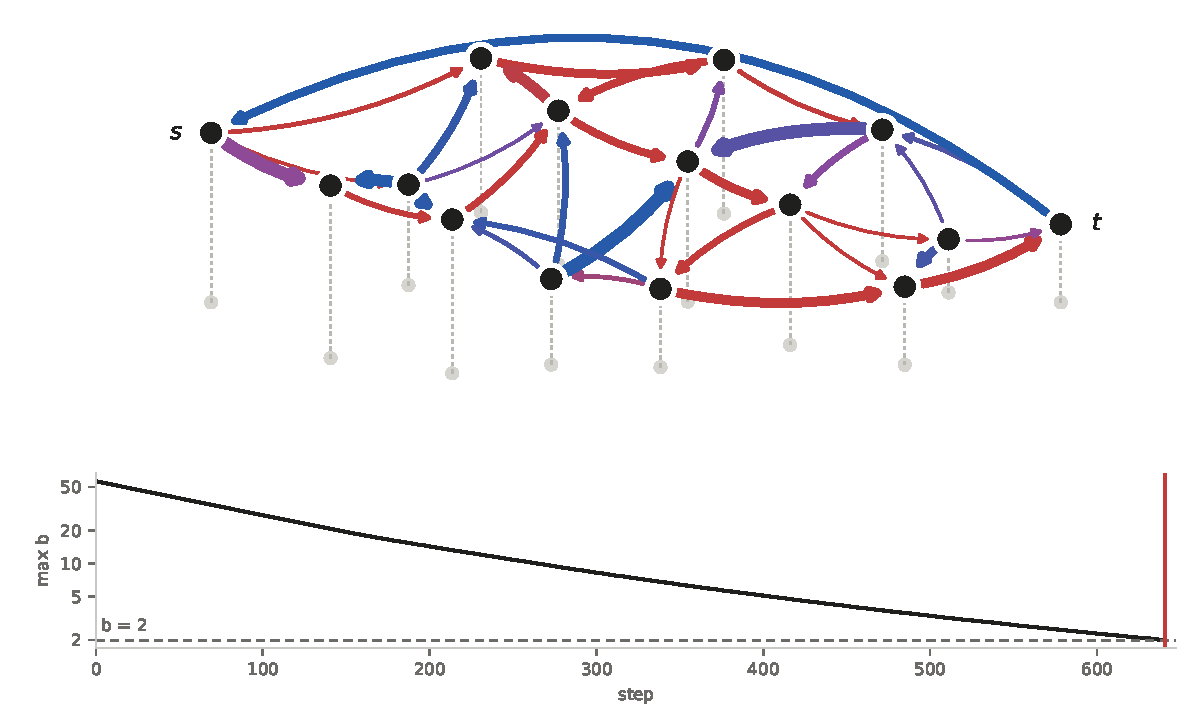
\includegraphics[width=0.85\linewidth]{viz/process-final}}
  \caption{
    The final frame of the process (click for the animation) on a random graph
    with $15$ vertices and capacities in $[1, 10]$, using the discrete steps of
    Section~\ref{sec:oracle} with $\epsilon = 1/4$. Blue vertices form the cut
    $S$ being raised. Arcs are colored by $f(u, v)/c(u, v)$, from blue ($0$)
    through purple to red ($1$, saturated), and thicker arcs have larger
    capacity. The arc arching from $t$ to $s$ stands for all $m = 33$ anchors.
    Below is the maximum of $b = f(\incut{S})/f(\outcut{S})$ over all cuts, with
    the current step marked; the process stops once it reaches $2$.
  }
  \label{fig:process}
\end{figure}

Let $y_\mu$ denote the potential at time $\mu$. If this process ever stops,
every $S$ must have $f(\incut{S})/f(\outcut{S}) \leq 2$ (i.e.\ we have a
$2$-pseudo-circulation), so we just need to argue that we terminate. For an edge
$(u, v)$, let $f_\Delta(u, v)$ denote the flow from $u$ to $v$ if
$y(v) - y(u) = \Delta$. Undecorated, $f(u, v)$ means the flow from $u$ to $v$ at
time $\mu$, i.e.\ $f_{y_\mu(v)-y_\mu(u)}(u, v)$. Consider the following
quantity:
\begin{align*}
  \mathcal{E}(\mu) \defeq \sum_{(u, v) \in E} \int_{y_\mu(v)-y_\mu(u)}^M f_\Delta(u, v) d\Delta,
\end{align*}
where $M = \max_{(u, v) \in E, \mu}\Set{y_\mu(v) - y_\mu(u)}$ (the integral
bounds ensure that $\mathcal{E} \geq 0$ at all times). Call this the ``energy''.
Viewed as a function of $y$, its derivative with respect to $y(w)$ is the net
outflow $f(\outcut{\Set{w}}) - f(\incut{\Set{w}})$ at $w$. So
$\nabla \mathcal{E} = 0$ exactly when $f$ is a circulation, and
$\langle \nabla \mathcal{E}, \mathbf{1}_S \rangle = f(\outcut{S}) - f(\incut{S})$.
Since $f_\Delta$ is nonincreasing in $\Delta$, $\mathcal{E}$ is also convex. The
process above is thus steepest descent on $\mathcal{E}$ over cut directions
$\mathbf{1}_S$ normalized by $f(\cut{S})$.

How does this quantity evolve?
\begin{align*}
  \frac{d\mathcal{E}}{d\mu} & = \sum_{(u, v) \in E} \frac{d}{d\mu}\paren{\int_{y_\mu(v)-y_\mu(u)}^{M} f_\Delta(u, v) d\Delta} \\
                            & = \sum_{(u, v) \in E} -f(u, v)\frac{d}{d\mu}\paren{y(v) - y(u)}                                 \\
                            & = \sum_{(u, v) \in E} f(u, v)\frac{d}{d\mu}\paren{y(u) - y(v)}.
\end{align*}
For edges $(u, v) \notin \cut{S}$ at time $\mu$, $y(u) - y(v)$ is constant. For
edges $(u, v) \in \outcut{S}$, $\frac{d}{d\mu}(y(u) - y(v)) = 1/f(\cut{S})$; for
$(u, v) \in \incut{S}, \frac{d}{d\mu}(y(u) - y(v)) = -1/f(\cut{S})$.

We then have
\begin{align*}
  \frac{d\mathcal{E}}{d\mu} & = \sum_{(u, v) \in E} f(u, v)\frac{d}{d\mu}\paren{y(u) - y(v)}                                                    \\
                            & = \sum_{(u, v) \in \outcut{S}} \frac{f(u, v)}{f(\cut{S})} - \sum_{(u, v) \in \incut{S}}\frac{f(u, v)}{f(\cut{S})} \\
                            & = \frac{f(\outcut{S}) - f(\incut{S})}{f(\cut{S})}.
\end{align*}
Since $f(\incut{S}) > 2f(\outcut{S})$, the final term is at most
\[
  \frac{\frac{1}{3}f(\cut{S}) - \frac{2}{3}f(\cut{S})}{f(\cut{S})} = -\frac{1}{3}.
\]
So the process terminates after at most $3\mathcal{E}(0)$ seconds. Since at
$\mu = 0$, $y(u) = 0$ for all $u \in V$,
\begin{align*}
  \mathcal{E}(0) & = \sum_{(u, v) \in E} \int_0^M f_\Delta(u, v) d\Delta                            \\
                 & = \sum_{(u, v) \in E} \int_0^M \frac{1}{\max\Set{\Delta, 0} + 1/c(u, v)} d\Delta \\
                 & = \sum_{(u, v) \in E} \ln(M + 1/c(u, v)) - \ln(1/c(u, v))                        \\
                 & \leq \sum_{(u, v) \in E} \ln(M + 1) + \ln(U) \leq 2m(\ln(M + 1) + \ln(U)),
\end{align*}
using $c(u, v) \geq 1$ and that the preprocessed graph has at most $2m$ arcs.

To show that the algorithm that simulates this process is efficient, we need to
argue that $\ln(M + 1) = \apxO{1}$. (Since $M$ is defined in terms of the whole
run, this might look circular. It isn't: $\frac{d\mathcal{E}}{d\mu}$ doesn't
depend on $M$, so we can run the argument below with $M$ replaced by the maximum
over any finite time window $[0, T]$, and the resulting bound doesn't depend on
$T$.) Let $(u^*, v^*)$ be an arc supporting $M$, so at some time $\mu^*$,
$y(v^*) - y(u^*) = M$. Since the preprocessed graph is strongly connected, there
is a path from $v^*$ to $u^*$ with at most $n - 1$ arcs. The potential
differences along it sum to $y(u^*) - y(v^*) = -M$, so some arc $(u, v)$ on it
has $y(v) - y(u) \leq -M/(n - 1) \leq -M/n$. That arc's contribution to the
energy is
\begin{align*}
  \int_{y_{\mu^*}(v)-y_{\mu^*}(u)}^M f_\Delta(u, v) d\Delta & \geq \int_{-M/n}^0 \frac{d\Delta}{\max\Set{0, \Delta} + 1/c(u, v)}                    \\
                                                            & = \int_{-M/n}^0 c(u, v)d\Delta                                                        \\
                                                            & = c(u, v)M/n \geq M/n                                              & (c(u, v) \geq 1)
\end{align*}
Every other arc contributes a nonnegative amount, and $\mathcal{E}$ decreases
throughout, so
\[
  M/n \leq \mathcal{E}(\mu^*) \leq \mathcal{E}(0) \leq 2m(\ln(M + 1) + \ln(U)).
\]
Let $A = 2nm$, so that $M \leq A\ln(M + 1) + A\ln(U)$. To solve this, use the
tangent-line bound $\ln z \leq \ln k + z/k - 1$ (concavity of $\ln$) with
$z = M + 1$ and $k = 2A$:
\[
  A\ln(M + 1) \leq A\ln(2A) + \frac{M + 1}{2} - A \leq A\ln(2A) + \frac{M}{2}.
\]
Substituting and rearranging, $M \leq 2A\ln(2A) + 2A\ln(U) = 4nm\ln(4nmU)$.
Since $n \leq 2m$, this gives $\ln(M + 1) = \bigO{\log(mU)}$, so
$\mathcal{E}(0) = \bigO{m\log(mU)}$, and the process terminates in time
$\bigO{m\log(mU)}$.

\subsection{Simulating with an Oracle}
\label{sec:oracle}

Of course, we can only simulate the process. Suppose we had an oracle that, for
a potential $y$, gave us the min-ratio cut $S$. For some step size
$\eta = \epsilon/f(\cut{S})$, we add $\eta$ to every $u \in S$. As is standard
in gradient descent, we need to prove that the gradient of $\mathcal{E}$ is
sufficiently Lipschitz. Consider a single iteration with cut $S$, and fix some
$(u, v) \in \incut S$. Let $\Delta$ represent the difference in their potentials
before the adjustment. The new flow on the arc is
\begin{align*}
  f_{\Delta+\eta}(u, v) & = \frac{1}{\max\Set{0, \Delta + \eta} + 1/c(u, v)}        \\
                        & \geq \frac{1}{1/f_\Delta(u, v) + \eta}                    \\
                        & = \frac{1}{1/f_\Delta(u, v) + \epsilon/f(\cut{S})}        \\
                        & \geq \frac{1}{1/f_\Delta(u, v) + \epsilon/f_\Delta(u, v)} \\
                        & = \frac{f_\Delta(u, v)}{1 + \epsilon}.
\end{align*}
Similarly, for any $(u, v) \in \outcut{S}$,
\[
  f_{\Delta-\eta}(u, v) \leq \frac{f_\Delta(u, v)}{1 - \epsilon}.
\]
And since $f_\Delta$ is monotone, it remains within a $\frac{1}{1 \pm \epsilon}$
factor of its starting point as $y(v) - y(u)$ is changed by $\pm \eta$.
Therefore, by picking a sufficiently small $\epsilon$ (say $1/8$), the
calculations for $\frac{d\mathcal{E}}{d\mu}$ go through nearly identically, and
we're left with a constant decrease in $\mathcal{E}$ in each step.

\subsection{An Approximate, Out-of-date Oracle}

The rest of this is really an implementation detail. (TODO)

\printbibliography
\end{document}
